\documentclass[11pt]{article}

\usepackage[margin=1in]{geometry}
\usepackage{amsmath}
\usepackage{amssymb}
\usepackage{booktabs}
\usepackage{array}
\usepackage{graphicx}
\usepackage{xcolor}
\usepackage{caption}
\usepackage[hidelinks]{hyperref}
\usepackage{microtype}
\usepackage{parskip}
\usepackage{enumitem}
\usepackage{float}

\newcommand{\win}{\textcolor{green!45!black}{$\blacktriangledown$}}
\newcommand{\loss}{\textcolor{red!70!black}{$\blacktriangle$}}
\newcommand{\tie}{\textcolor{gray}{$\bullet$}}
\newcommand{\dd}{$\Delta$}

\title{\textbf{Adaptive Multi-Timescale CTR Learning under Temporal Distribution
Shift}\\[4pt]
\large Findings Summary: AMG-TP versus Prior Adaptive-Training Methods}
\author{CTR-prediction-temporal-distribution-shift project}
\date{31 August 2026}

\begin{document}
\maketitle

\begin{abstract}
\noindent
This note summarises where the project stands after implementing and confirming
\textbf{AMG-TP} (Adaptive Multi-Timescale Gating with Temporal Persistence), and
collects the evidence bearing on the question \emph{does the new method
outperform the previous ones?} AMG-TP is a single causally-deployed model that
gates $K{=}5$ historical-horizon predictors per example and learns, with no
regime label, how much day-to-day inertia to impose on that mixture. Across a
eight-regime synthetic shift suite (12 disjoint confirmation seeds), two real
CTR datasets (Criteo, Avazu), and a frozen-model downstream autobidding
evaluation, AMG-TP \textbf{reproducibly beats the strongest prior baseline (Han
ARW)} on recurring, local, and opposing-local drift and on the real Avazu
stream, while \textbf{eliminating the abrupt-drift regression} that the best
previous project method (M5b-high-smooth) suffered. It does not dominate every
regime---the raw low-persistence gate is still slightly better under local
drift, and Han ARW is still better under gradual and mixed drift---so the result
is a \emph{partial success}: one adaptive model replaces a hand-tuned pair of
specialists and a three-way ensemble with little loss and no catastrophic
failure mode. Two extensions (per-example persistence $\beta_t(x)$; a
hidden-layer persistence network) remain untried and are the recommended next
step.
\end{abstract}

\section{Method Lineage}

The project has proceeded through a sequence of increasingly capable
adaptive-training methods, all evaluated in a single shared pipeline (identical
candidate bank, splits, seeds, and metrics), so the comparisons below are
apples-to-apples.

\begin{table}[H]
\centering
\small
\begin{tabular}{@{}lp{11.2cm}@{}}
\toprule
Method & Mechanism \\
\midrule
Expanding ERM & Retrain on all history each block. Strongest \emph{simple} fixed baseline. \\
Rolling-$h$ & Retrain on the last $h$ blocks ($h\in\{1,3,7,14\}$). \\
Han ARW & Adaptive global rolling window (Goldenshluger--Lepski selection). \textbf{Strongest prior adaptive baseline.} \\
AdaMoE, Diff.\ Forgetting & EMA expert weighting; learned exponential decay. \\
M1 & One global short/long mixing weight $\alpha_t$, grid-searched on recent matured days. \\
M2 & Per-example $\alpha_t(x)$ over 2 experts (short $=$ rolling-3, long $=$ expanding) via a small online context gate. \\
M5b & M2's online gate generalised to all 5 window experts; day-to-day smoothness penalty \texttt{smooth\_reg}. \\
M5b-high-smooth & M5b with \texttt{smooth\_reg}~$=0.1$ instead of $10^{-3}$: strong temporal persistence. Best previous \emph{fixed} configuration. \\
ensemble3 & Online 3-way meta-gate over \{M2, M5b-default, M5b-high-smooth\} final predictions. Diagnostic ceiling. \\
\midrule
\textbf{AMG-TP} & M5b's 5-expert context gate $q_t(x)$ \emph{plus} a learned scalar persistence $\beta_t$ that adaptively blends $q_t(x)$ with an EMA $m_{t-1}$ of recently deployed weights. \\
\bottomrule
\end{tabular}
\caption{The methods under comparison. AMG-TP is the current single-model
recommendation.}
\end{table}

\section{AMG-TP}

Maintain $K=5$ CTR predictors on horizons $\{1,3,7,14,\text{expanding}\}$ days
(here: 2-hour blocks). For example $x$ at block $t$:
\begin{align}
q_t(x)   &= \operatorname{softmax}\!\big(g_\phi(x,\, p^{(1:K)}_t(x),\, s_{t-1})\big)
           && \text{raw context gate (M5b's gate)}\\
m_t      &= (1-\rho)\,m_{t-1} + \rho\, \mathbb{E}_x[\pi_t(x)]
           && \text{persistent temporal state}\\
\beta_t  &= \sigma\!\big(r_\psi(s_{t-1})\big) \in [0,1]
           && \text{adaptive persistence (one global scalar / block)}\\
\pi_t(x) &= (1-\beta_t)\, q_t(x) + \beta_t\, m_{t-1}
           && \text{deployed temporal mixture}\\
\hat p_t(x) &= \textstyle\sum_{k} \pi_{t,k}(x)\, p^{(k)}_t(x).
\end{align}
The state $s_{t-1}$ (11 features) is built strictly from blocks $<t$: recent
per-expert loss, short/long disagreement, recent CTR, recent deployed gate
movement, normalised time, a loss-jump shift detector, and the divergence
between the last raw gate mean and $m_{t-1}$. Everything is causal: block $t$'s
prediction uses $q,\beta,m$ carried from blocks $<t$ only; $\phi,\psi,m$ update
after block $t$'s labels mature. Both networks are single linear layers,
zero-initialised, so AMG-TP starts as uniform expert averaging with
$\beta \approx \sigma(-1)$ and must \emph{learn} any adaptation. Parameter count
is negligible relative to the 5 SGD experts; ablation A9 (static uniform-5)
controls for model-count advantage.

\section{Experimental Setup}

\begin{itemize}[nosep]
\item \textbf{Synthetic suite S0--S7} (\texttt{synthetic\_data.py}): 120 blocks,
3000 rows/block. S0 stationary, S1 abrupt global, S2 gradual, S3 recurring
($A\!\to\!B\!\to\!A$, period 14), S4 local (one subgroup shifts), S5
opposing-local (two subgroups shift at different times), S6 mixed (random
sequence of shift types), S7 opposing-recurring (two subgroups oscillate a
quarter period out of phase; added in Stage 4, \S\ref{sec:s7}).
Hyperparameters frozen on 5 dev seeds
$\{0\text{--}4\}$; all results below are on \textbf{12 disjoint confirmation
seeds} $\{20\text{--}31\}$, reported as mean.
\item \textbf{Criteo} (31 days, full dataset, 3 SGD seeds): shallow natural
drift; treated as a no-downside check per plan \S5.3.
\item \textbf{Avazu} (\texttt{--source avazu}, 8 seeds): real 10-day mobile-ad
click logs, chronological stream rebuilt from the \texttt{hour} field, indexed
in 2-hour blocks, \texttt{id}/\texttt{hour} dropped so methods must find the
diurnal cycle from loss dynamics. Each seed draws a disjoint 20\% row
subsample. Second real benchmark per plan \S5.3.
\item \textbf{Downstream autobidding} (\texttt{autobid.py}, plan \S8): CTR
models frozen, each fed into the \emph{same} second-price auction $+$ per-block
pacing policy; primary metric is realised clicks at matched (25\%) spend.
Synthetic cost is tied to \emph{true} CTR, not to any model under test, so the
synthetic numbers measure whether a prediction gain \emph{translates}.
\end{itemize}
Pairing is by seed; CIs are paired bootstrap; $p$ is a Wilcoxon signed-rank test
across seeds ($p=0.000488$ is the floor for $n=12$; $p=0.0078$ the floor for
$n=8$).

\section{Results}

\subsection{Locked-test log loss by regime}

\begin{table}[H]
\centering
\footnotesize
\setlength{\tabcolsep}{4.2pt}
\begin{tabular}{@{}lrrrrrrrr@{}}
\toprule
regime & expand. & Han ARW & AdaMoE & M2 & M5b & M5b-hi & ens3 & \textbf{AMG-TP} \\
\midrule
S0 stationary      & \textbf{0.3270} & \textbf{0.3270} & 0.3543 & 0.3281 & 0.3282 & 0.3285 & 0.3281 & 0.3293 \\
S1 abrupt          & 0.5376 & 0.3389 & 0.3785 & 0.3983 & \textbf{0.3382} & 0.3467 & 0.3392 & 0.3389 \\
S2 gradual         & 0.4726 & \textbf{0.3581} & 0.3861 & 0.4045 & 0.3592 & 0.3618 & 0.3603 & 0.3603 \\
S3 recurring       & 0.4357 & 0.4368 & 0.4384 & 0.4333 & 0.4378 & 0.4275 & 0.4306 & \textbf{0.4298} \\
S4 local           & 0.5190 & 0.4885 & 0.5017 & 0.4879 & \textbf{0.4589} & 0.4671 & 0.4600 & 0.4612 \\
S5 opposing-local  & 0.6110 & 0.4947 & 0.5138 & 0.5354 & \textbf{0.4921} & 0.4966 & 0.4933 & 0.4936 \\
S6 mixed           & 0.5460 & \textbf{0.3919} & 0.4091 & 0.4300 & 0.3998 & 0.4019 & 0.4000 & 0.3975 \\
S7 opp.-recurring  & 0.4360 & 0.4360 & 0.4499 & 0.4340 & 0.4356 & \textbf{0.4326} & 0.4331 & 0.4359 \\
\midrule
Criteo (real)      & 0.6080 & 0.6072 & \textbf{0.6069} & 0.6072 & \textbf{0.6069} & 0.6070 & 0.6070 & \textbf{0.6069} \\
Avazu (real)       & 0.3844 & 0.3838 & 0.3826 & 0.3830 & 0.3826 & 0.3827 & 0.3826 & \textbf{0.3825} \\
\bottomrule
\end{tabular}
\caption{Mean locked-test log loss, confirmation seeds. M5b $=$
\texttt{m5b\_smooth0.001} (raw low-persistence gate); M5b-hi $=$
\texttt{m5b\_smooth0.1}. Bold $=$ best in row (within rounding). AMG-TP is
best or within noise of best in 6 of 10 rows; it is never the worst deployable
method in any row. S7 (added in Stage 4) is the exception discussed in
\S\ref{sec:s7}.}
\label{tab:headline}
\end{table}

\subsection{The headline evidence: AMG-TP versus Han ARW}

Han ARW is the strongest prior adaptive baseline and the reference the project
set out to beat. Table~\ref{tab:vshan} is the paired comparison.

\begin{table}[H]
\centering
\small
\begin{tabular}{@{}llrrrl@{}}
\toprule
regime & verdict & mean \dd{} log loss & rel.\ \% & seeds & Wilcoxon $p$ \\
\midrule
S3 recurring      & \win\ \textbf{AMG-TP wins}     & $-0.0070$ & $-1.60\%$ & 12/12 & $0.00049$ \\
S4 local          & \win\ \textbf{AMG-TP wins}     & $-0.0273$ & $-5.59\%$ & 12/12 & $0.00049$ \\
S5 opposing-local & \win\ AMG-TP wins (marginal)   & $-0.0011$ & $-0.22\%$ & 11/12 & $0.016$ \\
Avazu (real)      & \win\ \textbf{AMG-TP wins}     & $-0.0012$ & $-0.32\%$ & 8/8   & $0.0078$ \\
S1 abrupt         & \tie\ tie                      & $+0.0001$ & $+0.02\%$ & 5/12  & $0.79$ \\
S6 mixed          & \tie\ tie                      & $+0.0056$ & $+1.43\%$ & 5/12  & $0.38$ \\
S7 opp.-recurring & \tie\ tie (does not adapt)     & $-0.0001$ & $-0.01\%$ & 8/12  & $0.73$ \\
Criteo (real)     & \tie\ flat                     & $-0.0003$ & $-0.04\%$ & 3/3   & --- \\
S0 stationary     & \loss\ small loss             & $+0.0022$ & $+0.69\%$ & 0/12  & $0.00049$ \\
S2 gradual        & \loss\ small loss             & $+0.0022$ & $+0.62\%$ & 0/12  & $0.00049$ \\
\bottomrule
\end{tabular}
\caption{AMG-TP minus Han ARW, mean locked-test log loss. Negative $=$ AMG-TP
better. The stationary downside ($+0.0022$, $\approx 0.7\%$) is below the plan's
materiality bar; the gradual loss is the one genuine regression.}
\label{tab:vshan}
\end{table}

\noindent\textbf{Why this beats the previous project methods.} The earlier
method that beat Han ARW on recurring/local drift---M5b-high-smooth---did so at
the cost of a \textbf{+2.3\% regression on abrupt drift} (its heavy smoothing
reacts sluggishly to a step change). AMG-TP's learned $\beta_t$ removes that:

\begin{table}[H]
\centering
\small
\begin{tabular}{@{}lrrl@{}}
\toprule
regime & AMG-TP $-$ M5b (low-pers.) & AMG-TP $-$ M5b-hi (high-pers.) & reading \\
\midrule
S0 stationary      & $+0.0011$ & $+0.0008$ & matches both \\
S1 abrupt          & $+0.0007$ & $\mathbf{-0.0078}$ & \textbf{recovers the abrupt regression} \\
S2 gradual         & $+0.0011$ & $-0.0015$ & matches both \\
S3 recurring       & $\mathbf{-0.0081}$ & $+0.0023$ & captures most of the recurring gain \\
S4 local           & $+0.0023$ & $-0.0059$ & between them \\
S5 opposing-local  & $+0.0015$ & $-0.0030$ & between them \\
S6 mixed           & $-0.0024$ & $-0.0044$ & beats both \\
S7 opp.-recurring  & $+0.0003$ & $\mathbf{+0.0033}$ & \textbf{worse than both} \\
\bottomrule
\end{tabular}
\caption{AMG-TP versus the two fixed-persistence specialists it unifies
(confirmation seeds). A single learned $\beta_t$ recovers the low-persistence
specialist under abrupt/local/mixed drift \emph{and} the high-persistence
specialist under recurring drift, with no regime label. It does not
simultaneously beat \emph{both} in any single regime, and on S7---where the two
subpopulations want opposite persistence at every block---a single global
$\beta_t$ is worse than \emph{either} fixed choice (\S\ref{sec:s7}).}
\label{tab:specialists}
\end{table}

\noindent Against \textbf{ensemble3} (the diagnostic ceiling, a run-time 3-way
ensemble needing all three specialists), AMG-TP lands within $\pm0.003$ log loss
everywhere and actually beats it on S3 ($-0.0008$) and S6 ($-0.0026$). One
adaptive model reproduces a three-model ensemble.

\subsection{$\beta_t$ emerges correctly with no regime label (H2)}

\begin{table}[H]
\centering
\small
\begin{tabular}{@{}lrl@{}}
\toprule
regime & mean deployed $\beta_t$ & pre-shift $\to$ post-shift \\
\midrule
S0 stationary      & 0.43 & --- \\
S1 abrupt          & 0.36 & $0.41 \to 0.32$ \\
S2 gradual         & 0.45 & --- \\
S3 recurring       & \textbf{0.82} & --- \\
S4 local           & \textbf{0.27} & $0.41 \to 0.14$ \\
S5 opposing-local  & 0.33 & $0.39 \to 0.30$ \\
S6 mixed           & 0.36 & --- \\
S7 opp.-recurring  & 0.65 & --- \\
\bottomrule
\end{tabular}
\caption{Mean deployed $\beta_t$ ($0=$ trust the raw multiscale gate, $1=$ trust
the persistent state). High on recurring drift (persistence stabilises a smooth
cycle); collapses after the change point on abrupt/local drift (react fast,
discard a now-stale $m$). No drift label is ever given to $r_\psi$.}
\end{table}

\begin{figure}[H]
\centering
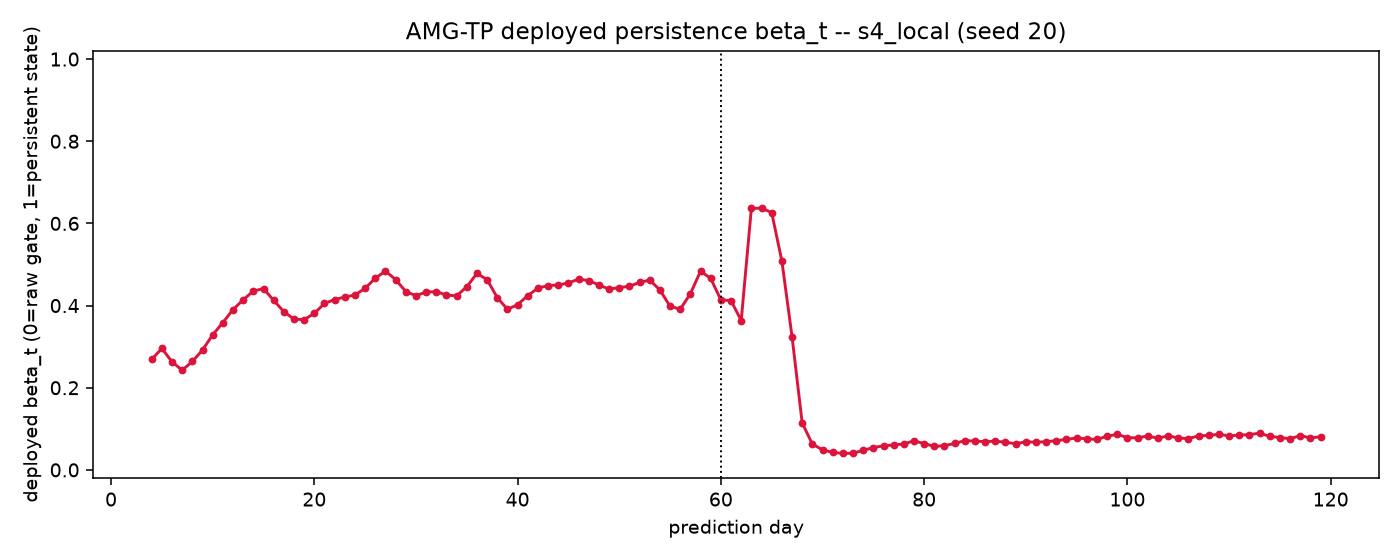
\includegraphics[width=0.49\textwidth]{stage2_amgtp/figures/beta_trace_s4_local.png}
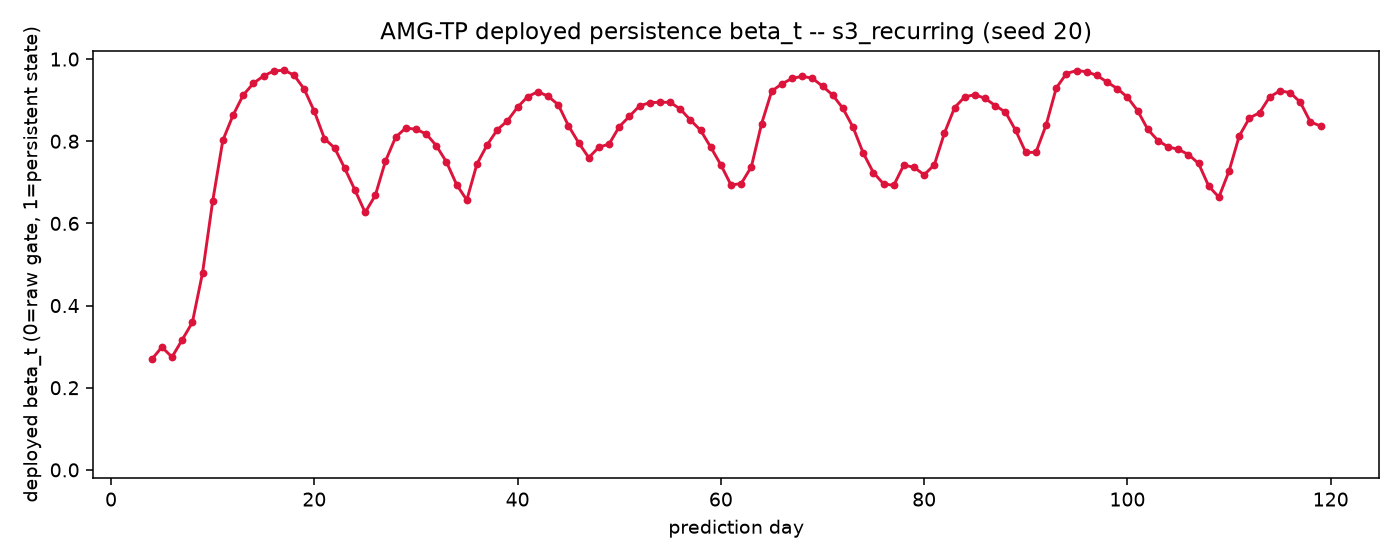
\includegraphics[width=0.49\textwidth]{stage2_amgtp/figures/beta_trace_s3_recurring.png}
\caption{Deployed $\beta_t$ over the prediction horizon. \emph{Left, S4 local:}
$\beta_t$ collapses from $\approx0.41$ to $\approx0.05$ within $\sim$8 blocks of
the shift. \emph{Right, S3 recurring:} $\beta_t$ stays high ($\approx0.8$)
throughout, holding the mixture stable across the cycle.}
\end{figure}

\subsection{Ablations (plan Table 3)}

\begin{table}[H]
\centering
\footnotesize
\setlength{\tabcolsep}{5pt}
\begin{tabular}{@{}llrrrrr@{}}
\toprule
ID & variant & S1 abrupt & S3 recur. & S4 local & S5 opp.-loc. & S7 opp.-recur. \\
\midrule
A0 & expanding only            & 0.5376 & 0.4357 & 0.5190 & 0.6110 & 0.4360 \\
A1 & no persistence ($\beta{=}0$) & 0.3382 & 0.4404 & 0.4590 & 0.4922 & 0.4356 \\
A3 & fixed high persistence    & 0.3467 & \textbf{0.4275} & 0.4671 & 0.4966 & \textbf{0.4326} \\
A4 & adaptive $\beta$, global $q$ (no context) & 0.3401 & 0.4312 & 0.4843 & 0.4940 & 0.4359 \\
A5 & adaptive $\beta$, uniform $q$ & 0.3817 & 0.4393 & 0.5040 & 0.5155 & 0.4510 \\
A6 & \textbf{full AMG-TP}      & 0.3389 & 0.4298 & \textbf{0.4612} & \textbf{0.4936} & 0.4359 \\
A7 & adaptive $\beta$, no state feats & 0.3388 & 0.4310 & 0.4629 & 0.4937 & 0.4354 \\
A9 & static uniform-5          & 0.3817 & 0.4393 & 0.5040 & 0.5155 & 0.4510 \\
A10 & nonlinear persistence net ($h{=}8$) & 0.3400 & 0.4258 & 0.4584 & 0.4987 & 0.4353 \\
\bottomrule
\end{tabular}
\caption{Ablation ladder, confirmation-seed mean log loss. The 5-expert
\emph{context} gate is essential (A5/A9 collapse under abrupt/local drift);
per-example context in $q$ matters most for local drift (A4 loses $0.023$ on
S4); adaptive $\beta$ is worth $\approx1\%$ on recurring versus $\beta{=}0$ (A1);
the state features give a small but consistent edge (A6 vs A7). \textbf{A10}
(Extension~A): a nonlinear hidden-layer persistence network, frozen on dev
seeds at width 0 after $h\in\{4,8,16\}$ never beat the linear net; it does not
change the picture on the confirmation seeds either---a validated negative
result.}
\end{table}

\subsection{Downstream autobidding: the prediction gains translate}

\begin{table}[H]
\centering
\small
\begin{tabular}{@{}llrrl@{}}
\toprule
regime & verdict & clicks @25\% spend, rel.\ \% vs Han ARW & seeds & $p$ \\
\midrule
S3 recurring      & \win\ \textbf{AMG-TP wins} & $+1.53\%$ & 8/8 & $0.008$ \\
S4 local          & \win\ \textbf{AMG-TP wins} & $+2.09\%$ & 8/8 & $0.008$ \\
S1 abrupt         & \tie\ tie ($+2.1\%$ vs M5b-hi) & $+0.17\%$ & 7/8 & $0.016$ \\
S5 opposing-local & \tie\ tie & $+0.12\%$ & 5/8 & $0.38$ \\
S0 / S2           & \loss\ small loss & $-0.31\%$ / $-0.25\%$ & 0/8 & $0.008$ \\
S6 mixed          & \loss\ loss & $-1.02\%$ & 0/8 & $0.008$ \\
Criteo (real)     & \tie\ flat & $+0.01\%$ & 4/5 & $0.125$ \\
\bottomrule
\end{tabular}
\caption{Realised value at matched spend, AMG-TP versus Han ARW, frozen models
into an unchanged bidder. The S3/S4 \emph{prediction} wins reproduce as
\emph{bidding-value} wins (plan Eq.~9 causal chain). On real Criteo nothing
separates from a cheapest-first bidder.}
\end{table}

\subsection{S7 opposing-recurring: where a global $\beta_t$ is not enough}
\label{sec:s7}

S7 (added in Stage 4) is a stress test of the single-global-persistence
assumption. Both subpopulations oscillate between the same two regimes with the
same period, but a \emph{quarter period out of phase}: at every block one group
sits near a turning point (its ground truth is momentarily stationary $\to$ high
persistence is optimal) while the other is at maximum slope (fast change $\to$
low persistence is optimal), and they trade roles continuously. Because the
schedule is cyclical rather than a one-off shift, this differential is present
in \emph{every} locked-test block, unlike S5 where it is a transient confined to
the development period.

The result (Table~\ref{tab:headline}, \ref{tab:specialists}): a single global
$\beta_t$ \textbf{cannot win here}. AMG-TP lands at $0.4359$---a dead tie with
Han ARW and plain expanding-history ERM ($-0.0001$, $p=0.73$), and
\emph{worse than either} fixed M5b specialist ($+0.0033$ vs high-persistence,
$+0.0003$ vs low). Adding per-example context to the gate does not rescue it
(A4 $\approx$ A6): the signal the model is missing is per-example
\emph{persistence}, not per-example \emph{horizon}. Yet the per-block oracle
shows the optimal fixed persistence flips on 66\% of test blocks, so the
headroom is real---it just requires $\beta$ to vary \emph{across examples},
which is exactly Extension~B.

\section{Does AMG-TP Outperform the Previous Methods?}

\begin{table}[H]
\centering
\small
\begin{tabular}{@{}llp{8.4cm}@{}}
\toprule
Hypothesis & Status & Evidence \\
\midrule
H1 adaptive memory scale & \textbf{supported} & Context gate $q_t(x)$ beats global/fixed horizons whenever the optimal horizon varies across examples (S4: A6 $0.461$ vs A4 no-context $0.484$; S5 similar). \\
H2 adaptive persistence & \textbf{supported} & One learned $\beta_t$ matches low-persistence M5b under abrupt/local and high-persistence M5b under recurring (Table~\ref{tab:specialists}), with no regime label; $\beta_t$ traces confirm the mechanism. \\
H3 low stationary downside & \textbf{supported} & S0: $+0.0022$ log loss ($+0.7\%$) vs expanding ERM---below the materiality bar. \\
H4 real CTR benefit & \textbf{weakly supported} & Avazu: beats Han ARW and expanding ERM $8/8$ seeds ($p=0.0078$); absolute effect small ($\sim$0.0012--0.0019). Criteo flat. \\
H5 downstream value & \textbf{partially supported} & S3 $+1.53\%$, S4 $+2.09\%$ clicks at matched spend, $8/8$ seeds. Real data does not separate. \\
\bottomrule
\end{tabular}
\end{table}

\noindent\textbf{Verdict (plan \S9): partial success $\to$ continue.} AMG-TP is
the recommended single model. Relative to prior methods:
\begin{itemize}[nosep]
\item versus \textbf{Han ARW}: reproducibly better on S3/S4/S5 and Avazu; ties
S1/S6/Criteo; small loss on S0/S2.
\item versus \textbf{M5b-high-smooth} (best previous fixed config): keeps most of
the recurring/local advantage and \emph{removes} the $+2.3\%$ abrupt-drift
regression.
\item versus \textbf{ensemble3} (3-way run-time ensemble): matched within
$\pm0.3\%$ everywhere with a single model; beats it on S3/S6.
\item versus \textbf{M5b-default / M2 / AdaMoE / diff.\ forgetting}: better or
tied in every synthetic regime and on both real datasets.
\end{itemize}

\noindent\textbf{Honest caveats.}
\begin{itemize}[nosep]
\item AMG-TP does not simultaneously beat \emph{both} fixed specialists in any
single regime---the raw low-persistence gate is still $\approx0.002$ better on
S4/S5, and M5b-high-smooth is $\approx0.002$ better on S3.
\item It still \emph{loses} to Han ARW on gradual (S2, $+0.6\%$) and does not
beat it on mixed (S6).
\item Real-data effects are small: Avazu $-0.32\%$, Criteo flat.
\item On \textbf{S7} a single global $\beta_t$ is worse than either fixed
persistence choice---the ``one model unifies the specialists'' story has a
boundary (\S\ref{sec:s7}).
\end{itemize}

\section{Extensions: Status and Next Steps}

Both extensions deferred by the plan (\S3) until the global-$\beta_t$ version was
understood are now in progress.

\paragraph{Extension A --- hidden-layer persistence network (done, negative).}
$r_\psi$ was a single linear layer; a tanh hidden layer (width $h$, zero-init
output so $h{=}0$ is bit-identical to Stage 2) was added and $h\in\{4,8,16\}$
swept on the dev seeds over S0/S1/S3/S4/S5/S7. No width beats the linear net on
summed dev log loss---deltas are fourth-decimal, worse on S1/S3, marginally
better on S5/S7---and the confirmation seeds agree (A10 in the ablation table).
Frozen at $h{=}0$; deployed AMG-TP is unchanged. Consistent with the Stage 2
finding that the persistence hyperparameters barely matter: the \emph{day-level}
state signal has no nonlinear structure worth the capacity.

\paragraph{Extension B --- per-example persistence $\beta_t(x)$ (next).}
Replace the scalar $\beta_t$ with
$\beta_t(x)=\sigma\big(r_\psi(s_{t-1}) + g_\xi(c(x))\big)$, $g_\xi$
zero-initialised so it collapses to the global value at init and only deviates
per example if that helps, with a variance penalty
$\lambda\,\mathrm{Var}_x[\beta_t(x)]$ for identifiability. \textbf{S7
opposing-recurring is the purpose-built test bed}: it is the one regime where a
global $\beta_t$ is provably wrong for one subpopulation at all times, where the
context gate $q_t(x)$ does not help, and where the per-block oracle still shows
66\% persistence-regime flips. Target: beat M5b-high-smooth's $0.4326$ on S7 by
giving each subpopulation its own persistence. Validated on the same
S0--S7 (dev $+$ confirm) $+$ Avazu $+$ Criteo battery with ablations A11--A13, a
per-group $\beta$ trace, and a per-group oracle-persistence diagnostic; if it
wins S7/S4/S5, the downstream autobidding evaluation is rerun. A $\beta_t(x)$
that merely ties the global version everywhere is itself a clean finding
(``$q_t(x)$ already absorbs per-example persistence''), closing plan \S3.

\vfill
\noindent\rule{\linewidth}{0.4pt}\\[2pt]
{\footnotesize Sources: \texttt{amgtp\_experiments/stage2\_amgtp/REPORT.md}
(S0--S7), \texttt{stage3\_autobid/REPORT.md},
\texttt{stage2\_amgtp/tables/ablation\_amgtp.csv},
\texttt{stage4\_hidden/\_sweep/FROZEN.md} (Extension A), and
\texttt{AMG-TP\_Academic\_LaTeX.pdf}. All synthetic numbers are means over the
12 confirmation seeds $\{20\text{--}31\}$; hyperparameters were frozen on dev
seeds $\{0\text{--}4\}$ before any confirmation run.}

\end{document}
